\section{Results}\label{sec:results}

\begin{table}[t]
\centering
\caption{Datasets after harmonisation. ``Rows read'' counts the records loaded; for CSE-CIC-IDS2018 it is the count after the 5\% Bernoulli subsampling of benign rows during streaming (all attack rows kept). ``Dup.'' is the share of those rows removed as exact duplicates over features and label. Benign and attack counts are after the per-class caps.}\label{tab:data}
\small
\begin{adjustbox}{max width=\linewidth}
\begin{tabular}{lrrrrrr}
\toprule
Dataset & Rows read & Unique & Dup. (\%) & Benign & Attack & Families\\
\midrule
\tabinput{tables/data.tex}
\bottomrule
\end{tabular}
\end{adjustbox}
\end{table}

\subsection{Data quality}
Table~\ref{tab:data} summarises the data. Exact duplicates are pervasive: between 26\% (CIC-IDS2017) and 56\% (ToN-IoT) of the records we loaded are feature-and-label copies of another record. Duplication is concentrated in a few families; for example, only 1{,}956 of the roughly 159{,}000 PortScan flows in our CIC-IDS2017 copy are unique, and only 54 of the 193{,}360 FTP-BruteForce flows in CSE-CIC-IDS2018 are unique. A random split of the raw data therefore places identical flows in the training and test sets, which inflates in-domain scores. All results below are computed after deduplication.

\subsection{In-domain performance is near ceiling and well calibrated}
In-domain, every model separates benign from attack traffic almost perfectly on the three CICFlowMeter datasets (Table~\ref{tab:xd}; AUROC 0.964--0.993) and on UNSW-NB15 and ToN-IoT (AUROC 0.964--1.000; per-model values are in the released result tables). The tree ensembles and the MLP are already well calibrated (ECE $\le 0.008$), and isotonic regression brings every model to ECE $\le 0.002$. The false-positive rate at the threshold chosen on the calibration split matches its nominal value ($\mathrm{FPR}/\alpha = 1.0$). Even here, however, the base rate caps what an alert can mean. At 1\% attack prevalence, a detector with 96\% TPR and 1\% FPR yields a precision of only about 0.49, so every second alert is a false alarm.

\begin{table}[t]
\centering
\caption{In-domain versus cross-dataset performance on the three CICFlowMeter datasets (mean $\pm$ s.d.\ over five seeds; cross-dataset values are averaged over the six directed pairs first). $\mathrm{FPR}/\alpha$ is the realised false-positive rate at the source threshold divided by its nominal value $\alpha=1\%$. TPR is measured at the same threshold. $\mathrm{Prec}_{1\%}$ is the precision implied at 1\% attack prevalence.}\label{tab:xd}
\small
\setlength{\tabcolsep}{3.5pt}
\begin{adjustbox}{max width=\linewidth}
\begin{tabular}{llcccccc}
\toprule
Model & Setting & AUROC & ECE (raw) & ECE (iso) & $\mathrm{FPR}/\alpha$ & TPR & $\mathrm{Prec}_{1\%}$\\
\midrule
\tabinput{tables/xd_main.tex}
\bottomrule
\end{tabular}
\end{adjustbox}
\end{table}

\subsection{Cross-dataset shift breaks ranking, calibration and alert volume at once}
Across datasets, all four models collapse to near-chance ranking (mean AUROC 0.50--0.62; Table~\ref{tab:xd}). The best pair, CIC-IDS2017$\to$CSE-CIC-IDS2018, reaches only 0.78 with LightGBM, and ACI-IoT-2023$\to$CIC-IDS2017 is \emph{worse} than chance (0.45; Fig.~\ref{fig:heat}). Individual seed--model runs range from AUROC 0.25 to 0.81, so the outcome of a single transfer experiment is largely a matter of chance. Calibration fails with the ranking: ECE rises from $\le0.04$ to 0.24--0.45, and isotonic or Platt recalibration fitted on source data does not help (isotonic ECE 0.28--0.45), because the mapping it learns belongs to the source distribution.

The operating point fails in two opposite ways that the ranking metrics hide. Models trained on CIC-IDS2017 or CSE-CIC-IDS2018 \emph{flood} a new network with alarms: their realised FPR is 5 to 32 times the nominal 1\% (Fig.~\ref{fig:heat}, right). Models trained on ACI-IoT-2023 instead go \emph{silent}: they keep the FPR near its nominal value on the other networks (1.2$\times$) but detect only 2--3\% of the attacks. The implied precision at 1\% prevalence falls from 0.39--0.49 in-domain to 0.024--0.034 across datasets, meaning that about 97 of every 100 alerts would be false. Per-group recall shows that sharing an attack name does not guarantee transfer. The CSE-CIC-IDS2018 model detects 76\% of CIC-IDS2017 DoS flows but only 0.2\% of its DDoS flows, and the CIC-IDS2017 model detects 70\% of CSE-CIC-IDS2018 DoS flows but 0.6\% of its botnet flows (released per-group table).

\begin{figure}[t]
\centering
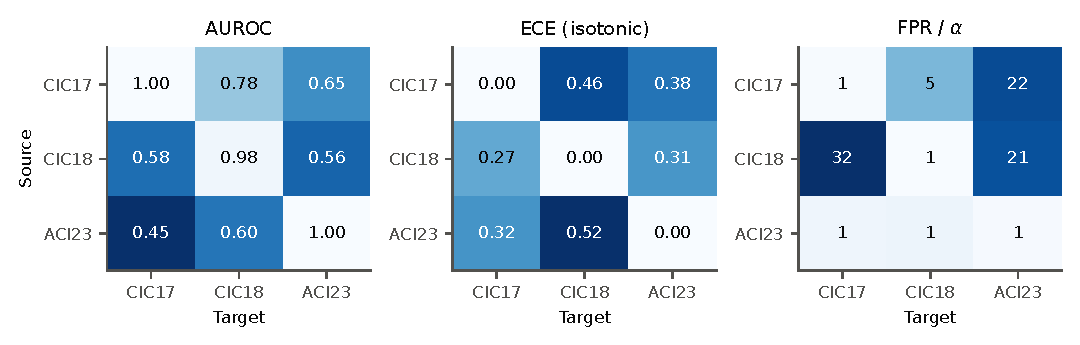
\includegraphics[width=\linewidth]{../figures/xd_heatmaps.pdf}
\caption{LightGBM trained on the row dataset and tested on the column dataset (mean over five seeds). Left: AUROC. Middle: ECE after isotonic calibration fitted on the source. Right: realised false-positive rate at the source threshold divided by the nominal 1\% (colour on a log scale). Diagonals are in-domain.}\label{fig:heat}
\end{figure}

\subsection{Unseen attack families are often missed, and missed confidently}
Holding out each of the 47 attack families with at least 300 flows, one at a time, lowers the median recall at the 1\% FPR threshold from 0.999 for the families seen in training to 0.847 for the held-out family (Table~\ref{tab:os}). The median hides a heavy tail: 14 of the 47 families (30\%) are detected less than half of the time. For 11 of them, more than half of the flows receive an isotonic-calibrated attack probability below 0.05, so the calibrated model is confidently wrong (Fig.~\ref{fig:os}). ACI-IoT-2023 is the extreme case: 7 of its 10 families fall below 50\% recall, and the median confident-miss rate is 0.96, because its floods and sweeps look nothing like the other attacks in the same dataset. CIC-IDS2017 Bot (recall 0.002) and SSH-Patator (0.09), CSE-CIC-IDS2018 Infiltration (0.03) and DDoS-LOIC-HTTP (0.03), and UNSW-NB15 Fuzzers (0.16) are other examples.

However, the information needed to find these flows is often present in the score. The AUROC between the held-out family and benign traffic stays high (median per dataset 0.90--0.996). The failure is therefore mainly one of \emph{thresholding}: the attack scores rise above benign scores, but not above a threshold tuned for the families the model already knows. This is what motivates reviewing flows by rank under a budget rather than by a fixed threshold.

\begin{table}[t]
\centering
\caption{Leave-one-family-out results with LightGBM (three seeds). Recall is measured at the source 1\%-FPR threshold. Median values are across held-out families. ``$<$0.5'' is the number of held-out families detected less than half of the time. ``Conf.\ miss'' is the median (maximum) fraction of held-out flows that the isotonic-calibrated model scores below 0.05. The two AUROC columns compare held-out flows with benign flows, using the detector score and the benign-referenced kNN novelty score respectively.}\label{tab:os}
\small
\setlength{\tabcolsep}{3.5pt}
\begin{adjustbox}{max width=\linewidth}
\begin{tabular}{lccccccc}
\toprule
Dataset & Fam. & Recall (seen) & Recall (unseen) & $<$0.5 & Conf.\ miss & AUROC det. & AUROC nov.\\
\midrule
\tabinput{tables/os_summary.tex}
\bottomrule
\end{tabular}
\end{adjustbox}
\end{table}

\begin{figure}[t]
\centering
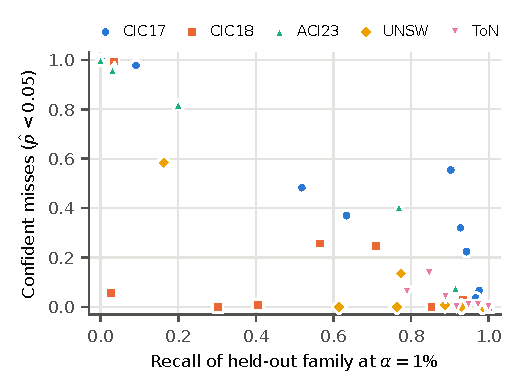
\includegraphics[width=0.62\linewidth]{../figures/os_scatter.pdf}
\caption{Each point is one held-out attack family (mean over three seeds). Points in the upper-left region are families the detector misses at its operating threshold \emph{and} labels benign with more than 95\% calibrated confidence.}\label{fig:os}
\end{figure}

\subsection{Budgeted triage}
Figure~\ref{fig:triage} and Table~\ref{tab:triage} report the fraction of attacks that land in the analyst queue when the queue holds the top 1\%, 2\% or 5\% of a stream with 1\% attack prevalence.

\paragraph{In-domain} Ranking by the detector score is best, capturing 89\%, 94\% and 96\% of attacks at the three budgets. Adding novelty evidence costs a little: Fisher fusion is lower by 2.5 points on average (Wilcoxon signed-rank $p<10^{-10}$ over 75 paired configurations), and novelty alone is poor (21--57\%), because known attacks need no novelty evidence.

\paragraph{Unseen families} Averaged over all 47 families, Fisher fusion and the detector score are statistically indistinguishable (mean difference $+1.0$ point, $p=0.29$ over 423 paired configurations). The average, however, mixes two groups with opposite behaviour (Table~\ref{tab:gain}). For the 14 families that the detector misses at its threshold, Fisher fusion doubles the recall inside a 1\% budget (0.072 to 0.152) and adds about 10 points at 2\% and 5\% ($p=4\times10^{-8}$; better in 68\% and worse in 20\% of paired configurations). For the 33 families the detector already catches, fusion costs up to 6 points at a 2\% budget. The Bonferroni rule is more conservative and brings no gain on either group. The grouping uses the held-out labels, so it explains where fusion helps but cannot serve as a deployment rule; Section~\ref{sec:discussion} discusses the trade-off.

\paragraph{Cross-dataset} No ranking rescues cross-dataset transfer. With a 5\% budget, every priority captures only 13--15\% of the attacks, against 5\% for a random queue of the same size.

\begin{figure}[t]
\centering
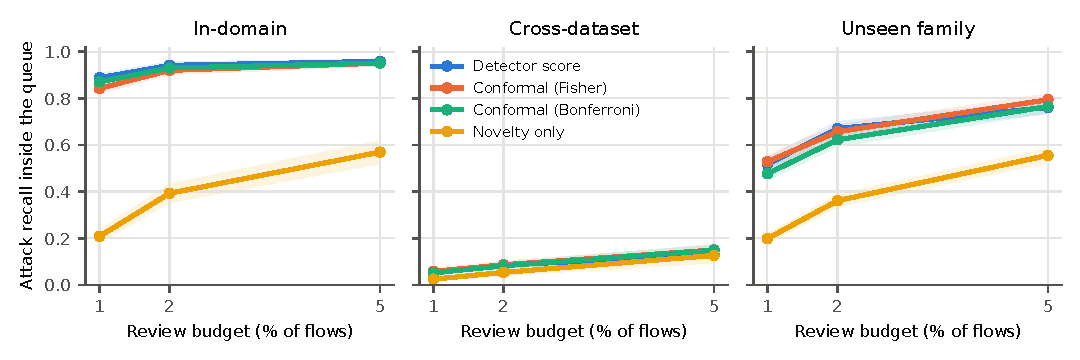
\includegraphics[width=\linewidth]{../figures/triage_recall.pdf}
\caption{Attack recall inside the review queue versus the review budget, for streams with 1\% attack prevalence (LightGBM; shaded bands are $\pm$1 standard error across configurations). The queue is the exact top-$b$ fraction of the stream by each priority.}\label{fig:triage}
\end{figure}

\begin{table}[t]
\centering
\caption{Attack recall inside the review queue (top-$b$ fraction of a stream with 1\% attack prevalence; LightGBM; mean over configurations).}\label{tab:triage}
\small
\begin{adjustbox}{max width=\linewidth}
\begin{tabular}{llccc}
\toprule
Regime & Priority & $b=1\%$ & $b=2\%$ & $b=5\%$\\
\midrule
\tabinput{tables/triage.tex}
\bottomrule
\end{tabular}
\end{adjustbox}
\end{table}

\begin{table}[t]
\centering
\caption{Unseen families: recall inside the queue, split by whether the detector's recall on the held-out family at the 1\%-FPR threshold is below 0.5. $\Delta$ is Fisher minus detector.}\label{tab:gain}
\small
\begin{adjustbox}{max width=\linewidth}
\begin{tabular}{lcccccc}
\toprule
Detector recall & Families & $b$ & Detector & Bonferroni & Fisher & $\Delta$\\
\midrule
\tabinput{tables/os_gain.tex}
\bottomrule
\end{tabular}
\end{adjustbox}
\end{table}

\subsection{Budgets can be enforced without target labels}
A review budget is only useful if the queue actually has the planned size. Table~\ref{tab:budget} and Fig.~\ref{fig:load} compare the two ways of setting the queue threshold for the Fisher priority. Transferring the threshold from the source works in-domain (median load 1.00--1.03). Under cross-dataset shift, the transferred threshold admits 20--54 times the planned volume at the median (the maximum possible load is $1/b$, i.e.\ the whole stream). The recall of 0.69--0.97 it reports in that setting is therefore an artefact of flagging almost everything. Under unseen-family shift, the transferred threshold instead leaves the queue at 38\% of its planned size at a 1\% budget and misses attacks the analysts had time to inspect. The label-free warm-up quantile keeps the median load between 0.98 and 1.05 in all three regimes (10th--90th percentile 0.84--1.34). With the queue size fixed, recall at a 1\% budget on unseen families rises from 0.41 to 0.53.

\begin{table}[t]
\centering
\caption{Budget adherence of the Fisher priority. ``Load'' is realised queue size divided by the planned size (median [10th, 90th percentile]); recall is attack recall inside the queue on the 80\% of the stream after the warm-up window.}\label{tab:budget}
\small
\setlength{\tabcolsep}{3pt}
\begin{adjustbox}{max width=\linewidth}
\begin{tabular}{llcccc}
\toprule
& & \multicolumn{2}{c}{Source threshold} & \multicolumn{2}{c}{Label-free warm-up}\\
\cmidrule(lr){3-4}\cmidrule(lr){5-6}
Regime & $b$ & Load & Recall & Load & Recall\\
\midrule
\tabinput{tables/budget.tex}
\bottomrule
\end{tabular}
\end{adjustbox}
\end{table}

\begin{figure}[t]
\centering
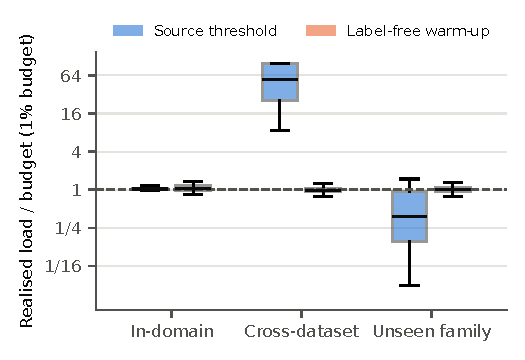
\includegraphics[width=0.55\linewidth]{../figures/budget_load.pdf}
\caption{Realised queue load relative to a 1\% review budget (log scale; 1 means the budget is met exactly). Transferred source thresholds overflow under cross-dataset shift and underfill under unseen-family shift; a quantile taken on the first 20\% of the unlabeled target stream holds the budget in every regime.}\label{fig:load}
\end{figure}

\subsection{Cost}
Scoring a flow with a detector plus the kNN novelty model takes a median of 35--40\,\textmu s per flow on four CPU cores, measured end to end in our Python pipeline, so the triage layer is cheap enough for flow-level deployment.
